\documentclass[10pt]{beamer}

% ------------------------------------------------------------------------
% Carga de tu preámbulo personalizado (preamble.tex).
% Recuerda colocarlo junto a este archivo para que \input funcione.
% ------------------------------------------------------------------------
\usetheme[progressbar=frametitle]{metropolis}
\usepackage{appendixnumberbeamer}
\usepackage{fancyvrb}
\usepackage{booktabs}
\usepackage[scale=2]{ccicons}
\usepackage{pgfplots}
\usepgfplotslibrary{dateplot}
\usepackage{type1cm}
\usepackage{lettrine}
\usepackage{ragged2e}
\usepackage{xspace}
\newcommand{\themename}{\textbf{\textsc{metropolis}}\xspace}
\usepackage{graphicx} % Allows including images
\usepackage{booktabs} % Allows the use of \toprule, \midrule and \bottomrule in tables
\usepackage[utf8]{inputenc} %solucion del problema de los acentos.
\usepackage{xcolor}
\definecolor{LightGray}{gray}{0.9}

\usepackage{minted}
\usemintedstyle{tango}
\newcommand{\mypyfile}[1]{\inputminted[linenos=true, fontsize=\footnotesize, frame=lines, framesep=5\fboxrule,framerule=1pt]{python}{#1}}

\setminted[python]{breaklines,frame=lines,framesep=2mm,baselinestretch=1.2,bgcolor=LightGray,linenos, fontsize=\footnotesize} % obeytabs=true, tabsize=2, showtabs=true}

%%%%%%%%%%%%%%%%%%%%%%%%%%%%%%%%%%%%%%%%%%%%%%%%%%%%%%%%%%%%%%%%%%%%%%%%%%%%%%%%%%%%%%
\setbeamercolor{progress bar}{fg=blue!50!black,bg=white!50!black}
\setbeamercolor{title separator}{fg=red!50!black,bg=white!50!black}
\setbeamercolor{frametitle}{fg=white!80!black,bg=red!50!black}
\title[PCFI161]{Programaci\'on para F\'isica y Astronom\'ia}
\subtitle{Departamento de Física.}

\newcommand{\myfront}{
\author[PCFI161]{Corodinadora: C Loyola \\ Profesoras/es C Loyola / C Femenías / Y Navarrete / C Ruiz}
\institute[UNAB]{Universidad Andrés Bello}
\date{Primer Semestre 2025}
}

\titlegraphic{%
  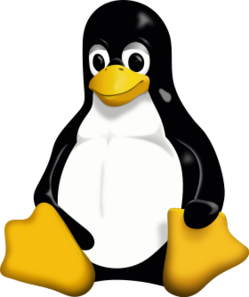
\includegraphics[width=.08\textwidth]{logo-tux.png}\hfill
  
\includegraphics[width=.3\textwidth]{logo-unab.png}\hfill
  
\includegraphics[width=.08\textwidth]{logo-python.png}
}

\makeatletter
\setbeamertemplate{title page}{
  \begin{minipage}[b][\paperheight]{\textwidth}
    \vfill%
    \ifx\inserttitle\@empty\else\usebeamertemplate*{title}\fi
    \ifx\insertsubtitle\@empty\else\usebeamertemplate*{subtitle}\fi
    \usebeamertemplate*{title separator}
    \ifx\beamer@shortauthor\@empty\else\usebeamertemplate*{author}\fi
    \ifx\insertdate\@empty\else\usebeamertemplate*{date}\fi
    \ifx\insertinstitute\@empty\else\usebeamertemplate*{institute}\fi
    \vfill
    \ifx\inserttitlegraphic\@empty\else\inserttitlegraphic\fi
    \vspace*{1cm}
  \end{minipage}
}
\makeatother


\makeatletter
\setlength{\metropolis@titleseparator@linewidth}{2pt}
\setlength{\metropolis@progressonsectionpage@linewidth}{2pt}
\setlength{\metropolis@progressinheadfoot@linewidth}{2pt}
\makeatother


\begin{document}

% ------------------------------------------------------------------------
% Portada de la Presentación
% ------------------------------------------------------------------------
\myfront{}

% ------------------------------------------------------------------------
% Slide 1: Título de la Sesión
% ------------------------------------------------------------------------
\begin{frame}
  \titlepage
  % Ejemplo:
  % \title{Semana 7 - Sesión 1 (Sesión 13): Gráficas Avanzadas con Matplotlib y Manipulación de Datos}
\end{frame}

% ------------------------------------------------------------------------
% Slide 2: Índice / Tabla de Contenidos
% ------------------------------------------------------------------------
\begin{frame}
  \frametitle{Resumen - Semana 7, Sesión 1 (Sesión 13)}
  \tableofcontents
\end{frame}

% ------------------------------------------------------------------------
% Configuración de bloques
% ------------------------------------------------------------------------
\metroset{block=fill}

% ----------------------------------------------------------------------------------------
% SECCIÓN 1: Introducción y Repaso de la Sesión Anterior
% ----------------------------------------------------------------------------------------
\section{Introducción y Repaso}

% ------------------------------------------------------------------------
% Slide 3: Repaso de la Sesión 12
% ------------------------------------------------------------------------
\begin{frame}{Repaso de la Sesión 12}
  \begin{itemize}
    \item \textbf{Semana 6, Sesión 2 (Sesión 12)} se enfocó en:
      \begin{itemize}
        \item Manipulación avanzada de NumPy (\texttt{reshape}, \texttt{transpose}, \texttt{concatenate}).
        \item Uso de \texttt{np.random} para valores aleatorios y \texttt{np.linalg} (álgebra lineal).
        \item Primeros pasos con \textbf{Matplotlib} (\texttt{plot}, \texttt{scatter}).
      \end{itemize}
    \item \textbf{Objetivo de hoy}: Avanzar con gráficos más complejos (subplots, histogramas, 3D) y comenzar a manipular datos de forma más eficiente (posiblemente una introducción a \texttt{pandas}).
  \end{itemize}
\end{frame}

% ------------------------------------------------------------------------
% Slide 4: Objetivos de la Sesión 13
% ------------------------------------------------------------------------
\begin{frame}{Objetivos de la Sesión 13}
  \begin{itemize}
    \item \textbf{Profundizar} en las opciones de \textbf{Matplotlib} para visualizar datos:
      \begin{itemize}
        \item Subplots, estilos, anotaciones.
        \item Gráficos de barras, histogramas y 3D simples.
      \end{itemize}
    \item \textbf{Familiarizarnos} con un primer acercamiento a \textbf{pandas}, si el tiempo lo permite.
    \item \textbf{Ejercitar} estos conceptos con ejemplos y datos relevantes para Física/Astronomía.
  \end{itemize}
\end{frame}

% ----------------------------------------------------------------------------------------
% SECCIÓN 2: Matplotlib Avanzado (Subplots, Barras, Histogramas)
% ----------------------------------------------------------------------------------------
\section{Matplotlib Avanzado}

% ------------------------------------------------------------------------
% Slide 5: Subplots Múltiples
% ------------------------------------------------------------------------
\begin{frame}[fragile]{Creando Varias Gráficas (Subplots)}
\begin{minted}{python}
import matplotlib.pyplot as plt
import numpy as np

x = np.linspace(0, 2*np.pi, 100)
y_sin = np.sin(x)
y_cos = np.cos(x)

fig, axs = plt.subplots(2, 1, figsize=(6,8))
axs[0].plot(x, y_sin, 'r-', label="sin(x)")
axs[0].legend()
axs[0].set_title("Seno")

axs[1].plot(x, y_cos, 'b--', label="cos(x)")
axs[1].legend()
axs[1].set_title("Coseno")

plt.tight_layout()
plt.show()
\end{minted}
\begin{itemize}
  \item \textbf{plt.subplots(rows, cols)}, retorna \textbf{fig} y un array de ejes \texttt{axs}.
  \item \texttt{plt.tight\_layout()} ayuda a optimizar la separación entre subplots.
\end{itemize}
\end{frame}

% ------------------------------------------------------------------------
% Slide 6: Gráficos de Barras
% ------------------------------------------------------------------------
\begin{frame}[fragile]{Gráficos de Barras}
\begin{minted}{python}
import matplotlib.pyplot as plt

etiquetas = ['A', 'B', 'C', 'D']
valores = [10, 25, 7, 15]

plt.bar(etiquetas, valores, color='lightblue')
plt.title("Gráfico de Barras")
plt.xlabel("Categorías")
plt.ylabel("Valores")
plt.show()
\end{minted}
\begin{itemize}
  \item Útil para datos categóricos o comparaciones discretas.
  \item \texttt{plt.barh} para barras horizontales.
\end{itemize}
\end{frame}

% ------------------------------------------------------------------------
% Slide 7: Histogramas
% ------------------------------------------------------------------------
\begin{frame}[fragile]{Histogramas}
\begin{minted}{python}
import numpy as np
import matplotlib.pyplot as plt

data = np.random.randn(1000)  # 1000 valores normal estándar
plt.hist(data, bins=20, color='green', alpha=0.7)
plt.title("Histograma de datos aleatorios")
plt.xlabel("Valor")
plt.ylabel("Frecuencia")
plt.show()
\end{minted}
\begin{itemize}
  \item \texttt{bins} controla el número de barras en el histograma.
  \item \textbf{alpha}: transparencia de las barras.
\end{itemize}
\end{frame}

% ----------------------------------------------------------------------------------------
% SECCIÓN 3: Gráficos 3D Básicos
% ----------------------------------------------------------------------------------------
\section{Gráficos 3D Básicos}

% ------------------------------------------------------------------------
% Slide 8: Módulo mpl\_toolkits.mplot3d
% ------------------------------------------------------------------------
\begin{frame}[fragile]{Instanciando Ejes 3D}
\begin{minted}{python}
from mpl_toolkits.mplot3d import Axes3D  # a partir de mpl_toolkits
import matplotlib.pyplot as plt
import numpy as np

fig = plt.figure()
ax = fig.add_subplot(111, projection='3d')
# ax ahora es un eje 3D
\end{minted}
\begin{itemize}
  \item Se puede usar \texttt{plt.subplots(subplot\_kw=\{'projection':'3d'\})} también.
  \item Métodos como \texttt{ax.plot3D}, \texttt{ax.scatter3D} están disponibles.
\end{itemize}
\end{frame}

% ------------------------------------------------------------------------
% Slide 9: Ejemplo de Superficie 3D
% ------------------------------------------------------------------------
\begin{frame}[fragile]{Plot de Superficie 3D (Ejemplo)}
\begin{minted}{python}
from mpl_toolkits.mplot3d import Axes3D
import matplotlib.pyplot as plt
import numpy as np

x = np.linspace(-5, 5, 50)
y = np.linspace(-5, 5, 50)
X, Y = np.meshgrid(x, y)
Z = np.sin(np.sqrt(X**2 + Y**2))

fig = plt.figure()
ax = fig.add_subplot(111, projection='3d')
ax.plot_surface(X, Y, Z, cmap='viridis')
ax.set_title("Superficie 3D")
plt.show()
\end{minted}
\begin{itemize}
  \item \texttt{plot\_surface}, \texttt{plot\_wireframe}, \texttt{plot\_contour}, etc.
\end{itemize}
\end{frame}

% ----------------------------------------------------------------------------------------
% SECCIÓN 4: Breve Introducción a Pandas (Opcional)
% ----------------------------------------------------------------------------------------
\section{Introducción a pandas (Opcional)}

% ------------------------------------------------------------------------
% Slide 10: ¿Por qué Pandas?
% ------------------------------------------------------------------------
\begin{frame}{¿Por qué pandas?}
  \begin{itemize}
    \item Librería para \textbf{manejo y análisis} de datos tabulares, muy usada en ciencia de datos.
    \item Estructuras \textbf{DataFrame} y \textbf{Series}.
    \item Integración con \textbf{NumPy} y \textbf{Matplotlib}.
    \item Lectura y escritura de archivos CSV, Excel, SQL, etc.
  \end{itemize}
\end{frame}

% ------------------------------------------------------------------------
% Slide 11: Ejemplo Rápido
% ------------------------------------------------------------------------
\begin{frame}[fragile]{Ejemplo Rápido con DataFrame}
\begin{minted}{python}
import pandas as pd

datos = {
    'Masa': [1.0, 3.5, 2.2],
    'Velocidad': [10.0, 7.5, 12.3]
}
df = pd.DataFrame(datos)
print(df)

# Calcular Energía Cinética
df['E_c'] = 0.5 * df['Masa'] * (df['Velocidad']**2)
print(df)
\end{minted}
\begin{itemize}
  \item Facilita manipulación de datos y operaciones columnares.
  \item \textbf{Opcional}: graficar \texttt{df['E\_c']} con \texttt{df.plot()} o \texttt{plt}.
\end{itemize}
\end{frame}

% ----------------------------------------------------------------------------------------
% SECCIÓN 5: Ejercicios y Actividad
% ----------------------------------------------------------------------------------------
\section{Ejercicios Prácticos}

% ------------------------------------------------------------------------
% Slide 12: Ejercicio 1 - Subplots
% ------------------------------------------------------------------------
\begin{frame}{Ejercicio 1: Subplots Seno, Coseno, Tangente}
  \begin{block}{Enunciado}
    \begin{itemize}
      \item Generar \texttt{x} en [0..2\(\pi\)], con \texttt{np.linspace}.
      \item Crear \textbf{3 subplots} en una columna:
        \begin{enumerate}
          \item \(\sin(x)\)
          \item \(\cos(x)\)
          \item \(\tan(x)\)
        \end{enumerate}
      \item Ajustar \textbf{ejes} y uso de \textbf{legends/titles}.
      \item Manejar la tangente en zonas cercanas a \(\pi/2\) (\textbf{ver si se disparan valores}).
    \end{itemize}
  \end{block}
\end{frame}

% ------------------------------------------------------------------------
% Slide 13: Ejercicio 2 - Histograma vs. Barras
% ------------------------------------------------------------------------
\begin{frame}{Ejercicio 2: Comparando Histogramas y Barras}
  \begin{block}{Enunciado}
    \begin{itemize}
      \item Generar 100 valores aleatorios con \texttt{np.random.normal(5,1,100)} (media=5, sigma=1).
      \item Hacer un \textbf{histograma} de esos datos (\texttt{plt.hist}).
      \item Contar manualmente las frecuencias en cada bin, y crear un \textbf{gráfico de barras} para comparar.
      \item Observar similitudes y diferencias.
    \end{itemize}
  \end{block}
  \textbf{Objetivo}: Entender la relación entre un histograma y los datos de frecuencia.
\end{frame}

% ------------------------------------------------------------------------
% Slide 14: Ejercicio 3 - Gráfico 3D
% ------------------------------------------------------------------------
\begin{frame}{Ejercicio 3: Gráfica 3D de una Función}
  \begin{block}{Enunciado}
    \begin{itemize}
      \item Definir una \textbf{función} \(f(x,y) = e^{-x^2 - y^2}\) (campana).
      \item Usar \texttt{np.meshgrid} para crear \(\texttt{X}, \texttt{Y}\) en [-2,2].
      \item Calcular \texttt{Z = f(X,Y)}.
      \item Crear un \textbf{plot de superficie} (\texttt{ax.plot\_surface}) con un color map bonito.
    \end{itemize}
  \end{block}
  \textbf{Sugerencia}: Ajustar \textbf{figsize} y \texttt{ax.set\_zlim} para ver mejor la forma.
\end{frame}

% ------------------------------------------------------------------------
% Slide 15: Ejercicio 4 (Opcional) - Leyendo Datos con pandas
% ------------------------------------------------------------------------
\begin{frame}{Ejercicio 4 (Opcional): Leyendo Datos con pandas}
  \begin{block}{Enunciado}
    \begin{itemize}
      \item Tener un archivo CSV simple con columnas: \texttt{Tiempo, PosX, PosY} (p.e., trayectoria de un objeto).
      \item Usar \texttt{pandas.read\_csv('archivo.csv')} para cargarlo a un DataFrame.
      \item Graficar \texttt{PosY} vs. \texttt{Tiempo} con \textbf{Matplotlib}.
      \item Agregar \textbf{labels} y título.
    \end{itemize}
  \end{block}
  \textbf{Objetivo}: Introducir la idea de leer datos externos y visualizar.
\end{frame}

% ------------------------------------------------------------------------
% Slide 16: Trabajo Colaborativo en Clase
% ------------------------------------------------------------------------
\begin{frame}{Trabajo Colaborativo}
  \begin{itemize}
    \item Dividir en \textbf{parejas} o \textbf{tríos}.
    \item Cada grupo elige \textbf{2-3 ejercicios} según interés.
    \item Implementar y analizar resultados en un \textbf{notebook de Colab}.
    \item Compartir conclusiones y dificultades al final.
  \end{itemize}
\end{frame}

% ------------------------------------------------------------------------
% Slide 17: Sugerencias y Tips
% ------------------------------------------------------------------------
\begin{frame}{Sugerencias y Tips}
  \begin{itemize}
    \item Para \textbf{subplots} múltiples, considerar \(\texttt{figsize}\) y \texttt{tight\_layout}.
    \item En \textbf{3D}, probar otras funciones como \(\cos(\sqrt{x^2 + y^2})\) o \(\sin(x*y)\).
    \item En \textbf{pandas}, puedes usar \texttt{df.describe()} para ver estadísticas rápidas.
    \item Explorar \textbf{paletas de colores}: \(\texttt{cmap='plasma'}\), \(\texttt{cmap='coolwarm'}\), etc.
  \end{itemize}
\end{frame}

% ------------------------------------------------------------------------
% Slide 18: Espacio para Dudas
% ------------------------------------------------------------------------
\begin{frame}{Espacio para Dudas}
  \begin{itemize}
    \item ¿Alguna confusión con \textbf{subplots} o configuración de ejes?
    \item ¿Problemas para instalar o importar \textbf{pandas}?
    \item ¿Dudas sobre gráficos 3D y el uso de \(\texttt{meshgrid}\)?
  \end{itemize}
  \vspace{0.2cm}
  \textbf{Levanta la mano o consulta abiertamente para que todos aprendan.}
\end{frame}

% ----------------------------------------------------------------------------------------
% SECCIÓN 6: Conclusiones y Próximos Pasos
% ----------------------------------------------------------------------------------------
\section{Conclusiones y Próximos Pasos}

% ------------------------------------------------------------------------
% Slide 19: Discusión de Soluciones
% ------------------------------------------------------------------------
\begin{frame}{Discusión de Soluciones}
  \begin{itemize}
    \item Comparte tus resultados en \textbf{subplots}, \textbf{histogramas} o \textbf{3D}.
    \item Si usaste \textbf{pandas}, ¿cómo fue la experiencia de cargar datos y manipularlos?
    \item Observa \textbf{beneficios} de la visualización en la interpretación de datos físicos/matemáticos.
  \end{itemize}
\end{frame}

% ------------------------------------------------------------------------
% Slide 20: Conclusiones de la Sesión 13
% ------------------------------------------------------------------------
\begin{frame}{Conclusiones de la Sesión 13}
  \begin{itemize}
    \item \textbf{Matplotlib avanzado}:
      \begin{itemize}
        \item Subplots múltiples, histogramas, barras, y nociones 3D.
      \end{itemize}
    \item \textbf{Breve introducción} a \texttt{pandas} para datos tabulares.
    \item Integramos \textbf{NumPy, Matplotlib} y (opcionalmente) \textbf{pandas} para un flujo de trabajo más completo.
    \item Seguiremos perfeccionando la \textbf{visualización} y manipulación de datos en las próximas sesiones.
  \end{itemize}
\end{frame}

% ------------------------------------------------------------------------
% Slide 21: Próxima Sesión
% ------------------------------------------------------------------------
\begin{frame}{Próximos Temas}
  \begin{itemize}
    \item \textbf{Semana 7, Sesión 2}: Profundizaremos en \textbf{visualizaciones personalizadas} (títulos, ejes, anotaciones, múltiples figuras) y exploraremos más sobre \textbf{manejo de datos}.
    \item Revisaremos \textbf{buenas prácticas} para proyectos colaborativos y la combinación de Python con LaTeX (si alcanza el tiempo).
  \end{itemize}
  \vspace{0.3cm}
  \textbf{Sigan practicando con datos reales o simulados para afianzar los conocimientos.}
\end{frame}

% ------------------------------------------------------------------------
% Slide 22: Recursos Adicionales
% ------------------------------------------------------------------------
\begin{frame}{Recursos Adicionales}
  \begin{itemize}
    \item \href{https://matplotlib.org/stable/}{\textbf{Matplotlib Docs}} (especialmente ejemplos de galería).
    \item \href{https://pandas.pydata.org/}{\textbf{pandas Documentation}} (guía de 10 minutos).
    \item \href{https://seaborn.pydata.org/}{\textbf{Seaborn}} (librería de visualización avanzada sobre Matplotlib).
    \item \href{https://docs.python.org/3/library/}{\textbf{Python Standard Library}} - repaso general.
  \end{itemize}
\end{frame}

% ------------------------------------------------------------------------
% Slide 23: Cierre de la Sesión
% ------------------------------------------------------------------------
\begin{frame}
  \Huge{\centerline{¡Gracias y hasta la próxima sesión!}}
  \vspace{0.4cm}
  \normalsize
  \begin{itemize}
    \item Recuerden subir sus notebooks y experimentos a Google Drive o repositorio compartido.
    \item Practiquen diferentes tipos de gráficos e integren datos con \textbf{pandas} si pueden.
  \end{itemize}
\end{frame}

\end{document}

